\documentclass[twoside]{article}
\usepackage[obeyspaces]{url}
\usepackage{natbib}
%\usepackage{chem}
\usepackage{color}
\usepackage{rotating} % loads graphicx
%\usepackage{longtable}
\usepackage{graphicx}
%\usepackage{verbatim}
%\usepackage{draftwatermark}\SetWatermarkScale{6}

\usepackage[nottoc]{tocbibind}
\settocbibname{References}          %%% Title of bibliography

\oddsidemargin-5mm
\evensidemargin-5mm
\topmargin-15mm
\textheight240mm
\textwidth175mm
\raggedbottom
\parindent0mm
\parskip1.0ex plus0.5ex minus0.5ex
\renewcommand{\arraystretch}{1}
\renewcommand{\topfraction}{0.95}
\renewcommand{\dbltopfraction}{0.95}
\renewcommand{\bottomfraction}{0.95}
\renewcommand{\floatpagefraction}{0.95}
\renewcommand{\dblfloatpagefraction}{0.95}
\renewcommand{\textfraction}{0.01}
\setcounter{topnumber}{3}
\setcounter{secnumdepth}{4}
\setcounter{tocdepth}{4}

\newcommand{\egcite}[1]{\citep[e.g.][]{#1}}
\newcommand{\etccite}[1]{\citep[and references therein]{#1}}
\newcommand{\hhline}{\noalign{\vspace{1mm}}\hline\noalign{\vspace{1mm}}}
\newcommand{\hhlines}{\noalign{\vspace{1mm}}\hline\hline\noalign{\vspace{1mm}}}
\newcommand{\kpproot}{{\sc root}}
\newcommand{\todo}[1]{{\uppercase{\bf ((#1))}}}

\def\mypageheader{A. Kerkweg et al.: AVEOUT User Manual}
\markboth{\mypageheader}{\mypageheader}
\pagestyle{myheadings}

\begin{document}

\thispagestyle{empty}
\vspace*{2.5cm}
%\vspace*{-2cm}
\begin{center}
  {\Huge\bf User Manual}\\[3mm]
  {\huge\it for the MESSy submodel}\\[3mm]
   {\Huge\bf AVEOUT}\\[27mm]
%%  {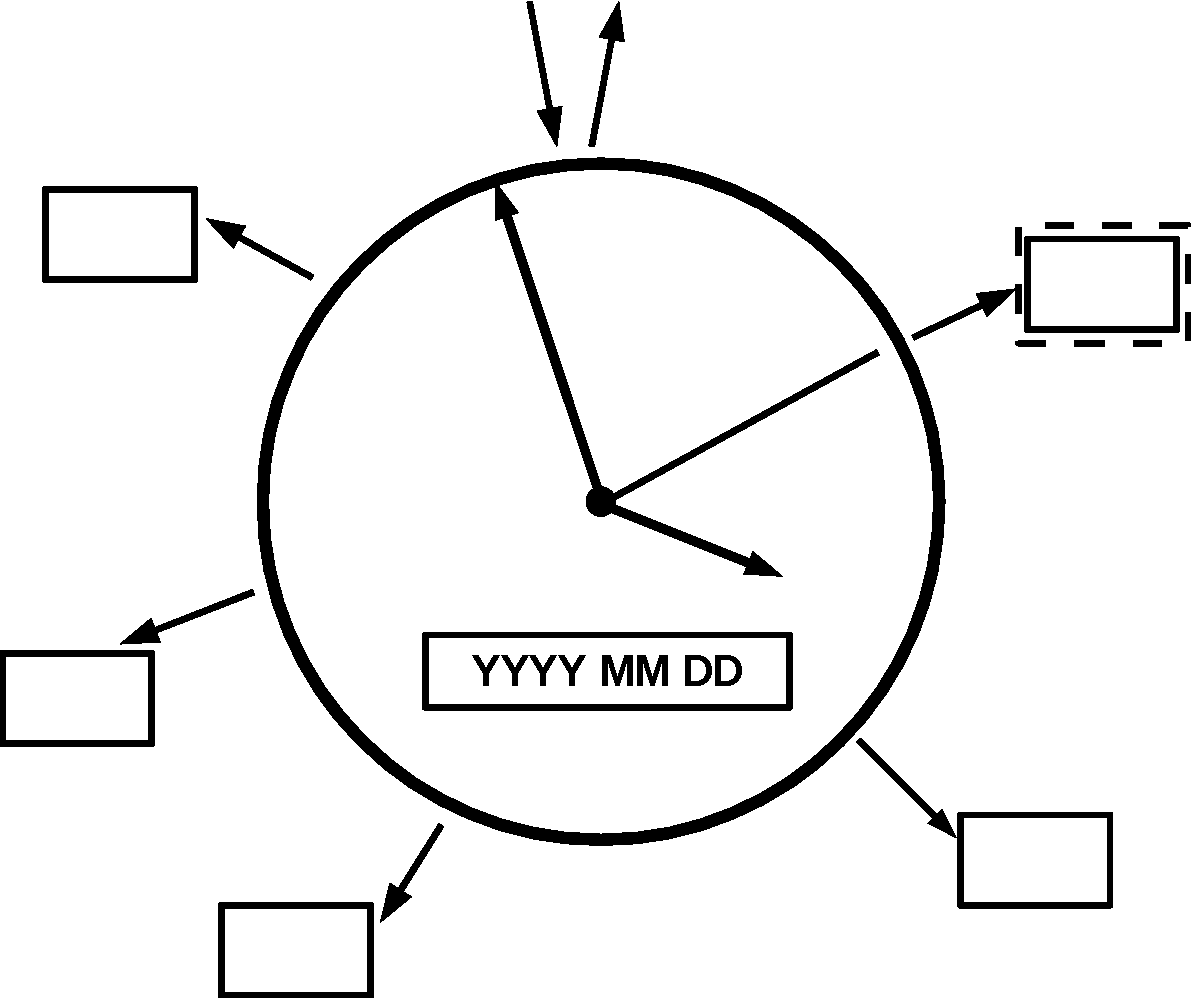
\includegraphics[width=0.7\textwidth]{timer_logo}}\\[9mm]
  {\huge\bf Astrid Kerkweg}\\[9mm]
  \normalsize
  Institute for Energy and Climate Research, Troposphere\\ Research Center
  J\"ulich, 52425 J\"ulich, Germany\\
  \url{a.kerkweg@fz-juelich.de}\\[3mm]
\end{center}

%\vfill
\vspace{4cm}
\tableofcontents
%% {\large This manual is part of the electronic supplement of our article
%% ``Development Cycle 2 of the Modular Earth Submodel System (MESSy2)''
%%   in Geosci.\ Model\ Dev.\
%%   (2010), available at: \url{http://www.geoscientific-model-development.net}}
\vspace{2cm}

\begin{center}
  Date: \today
\end{center}

%\newpage
%\tableofcontents
%\newpage

\newpage%\twocolumn
\sloppy

%%%%%%%%%%%%%%%%%%%%%%%%%%%%%%%%%%%%%%%%%%%%%%%%%%%%%%%%%%%%%%%%%%%%%%%%%%%%%%
%% ###########################################################################
%%%%%%%%%%%%%%%%%%%%%%%%%%%%%%%%%%%%%%%%%%%%%%%%%%%%%%%%%%%%%%%%%%%%%%%%%%%%%%
\section{Introduction}
\label{sec:intro}
%%%%%%%%%%%%%%%%%%%%%%%%%%%%%%%%%%%%%%%%%%%%%%%%%%%%%%%%%%%%%%%%%%%%%%%%%%%%%%
%% ###########################################################################
%%%%%%%%%%%%%%%%%%%%%%%%%%%%%%%%%%%%%%%%%%%%%%%%%%%%%%%%%%%%%%%%%%%%%%%%%%%%%%
%
Most Earth (Sub-)System Models provide instantaneous output of most variables,
but require hard-coded programming of other statistical (w.r.t. time)
measures, such as averages, maxima or minima over a specific time interval.
Thus for most Model Intercomparison Projects (MIPs), statistical measures
w.r.t. time (e.g., monthly averages, minima or maxima) are calculated on the
basis of regular instantaneous output (e.g., based on 3-hourly data).  The
statistical measures calculated by this procedure, however, deviate from
corresponding statistics, which are based on every time step.

In contrast to most other models, the generic MESSy submodel
CHANNEL enables a namelist driven output control of variables allowing to
choose by namelist, whether 1) a variable is written to the output, and 2) which
statistical measures (w.r.t. time) of the variable are output.
Here, the instantaneous value, the average, the standard
deviation, the minimum, the maximum and other measures w.r.t. the output
interval can be chosen independently. Since all time steps are taken into
account, the results differ from the corresponding statistical measures
calculated off-line from only a subset of time steps.

A thorough analysis, if and how much the statistics based on a subset of
time steps deviates from that based on all time steps is only possible,
if these measures are calculated within the same model. Sofar, a systematic
analysis of such deviations for longer simulation periods was hampered by the
need to output the instantaneous data each model time step over the entire
period.
However, with the MESSy submodels CHANNEL and AVEOUT, it is now possible to
output the statistical values calculated from each time step (CHANNEL),
and calculated from a regularly sampled subset of time steps (AVEOUT).
In the namelist of AVEOUT, variables and corresponding time intervals for
subsampling can be selected.

Section \ref{sec:idea} of this manual explains the technical background of
AVEOUT, i.e. how it is possible to mimic averaging of subsampling data in
time online. In Sect.\ \ref{sec:namelists} the required settings of the AVEOUT
and CHANNEL namelists are described. Last but not least, Sect.\ 4 shows a
first, sketchy analysis of the systematic errors introduced by using
subsampling in time for the calculation of statistical measures.

%%%%%%%%%%%%%%%%%%%%%%%%%%%%%%%%%%%%%%%%%%%%%%%%%%%%%%%%%%%%%%%%%%%%%%%%%%%%%%
%% ###########################################################################
%%%%%%%%%%%%%%%%%%%%%%%%%%%%%%%%%%%%%%%%%%%%%%%%%%%%%%%%%%%%%%%%%%%%%%%%%%%%%%
\section{How to imitate x-hourly data?}
\label{sec:idea}
%%%%%%%%%%%%%%%%%%%%%%%%%%%%%%%%%%%%%%%%%%%%%%%%%%%%%%%%%%%%%%%%%%%%%%%%%%%%%%
For the calculation of the statistical measures (w.r.t. time) in CHANNEL, all
time steps are taken into account. For time averages, for instance, results
after each time step are summed, and divided by the number of time steps just
before the output. For minima and maxima over time, the value after each time
step is compared to the sofar smallest or largest number and a new minimum or
maximum is determined. In the following, the explanation is provided for
averages only, as the minima and maxima calculation follows the same principle.

The off-line calculation is performed in basically the same way: For the
averages all available data values are summed, and the sum is
divided by the number of available data points.
The latter is, however, smaller, if the output was not written every time step.

As an example, the monthly mean surface temperature is calculated for
January, with a model time step length of 15 minutes on-line,
or off-line based on 3-hourly output:
%
In CHANNEL data of each time step, i.e., in sum 4 * 24 * 31 = 2976 data
points in time are taken in account, while in the off-line approach 1/3 * 24 *
31 = 248 data points are considered. The latter result remains the same,
if each 3-hourly value is considered 12 times, i.e.
the number of model time steps performed in 3 hours simulated time, and
divided by 2976 in the end. 

This is what AVEOUT does. It uses the CHANNEL output control, which sums up
each time step, but it provides the infrastructure to ensure that the
respective variable is only updated in a subset of time steps.
In this way, the averages calculated from subsets of time steps
can be directly compared to the averages calculated from all
instantaneous values. The latter is considered to be the ``truth'' in the
analysis in Sect.\ \ref{sec:results}.


%%%%%%%%%%%%%%%%%%%%%%%%%%%%%%%%%%%%%%%%%%%%%%%%%%%%%%%%%%%%%%%%%%%%%%%%%%%%%%
%% ###########################################################################
%%%%%%%%%%%%%%%%%%%%%%%%%%%%%%%%%%%%%%%%%%%%%%%%%%%%%%%%%%%%%%%%%%%%%%%%%%%%%%
%%%%%%%%%%%%%%%%%%%%%%%%%%%%%%%%%%%%%%%%%%%%%%%%%%%%%%%%%%%%%%%%%%%%%%%%%%%%%%
\section{Required namelist settings of AVEOUT and CHANNEL}
\label{sec:namelists}
%%%%%%%%%%%%%%%%%%%%%%%%%%%%%%%%%%%%%%%%%%%%%%%%%%%%%%%%%%%%%%%%%%%%%%%%%%%%%%

Figure \ref{fig:nml} shows an example for an AVEOUT \verb|&CPL| namelist. In
this example, the variable \verb|tm1|, i.e., the temperature from the
\verb|ECHAM5| channel is
processed to produce x-hourly output. Here the results are subsampled every
1st, 2nd, 3rd, 4th, 5th, 6th, 7th, 8th, 9th, 10th, 11th ,12th , 13th, 15th and
17th hour. Additionally, the 6-hourly sampling is shifted by
0, 1, 2, 3, 4 and 5 hours, respectively\footnote{in the MESSy TIMER submodel,
  the event shifting needs to be defined in seconds}.

The format of the namelist entries follows the typical MESSy syntax. The
channel object is determined by naming the channel and the object name.
For  models with patches or sub-domains, i.e.\ currently the ICON model,
the respective domains can be chosen by adding them via a comma separated list
to the channel 
name, e.g.:
\begin{verbatim}
 OUTPUT(12)='ICON:D01,D02','pres',3,'steps','first',0,
\end{verbatim}

The last 4 entries are the typical TIMER event control quadruplet. It can be
defined in units of 'steps', 'minutes', 'hours', 'days','months' and
'years'. The number in front of the unit string defines the length of the
interval in these units, and the last number defines the off-set in
seconds. For more information see the TIMER manual.

The actual output is controlled by the CHANNEL namelists. First,
it is required to determine, which statistical measure should be written
out. Either, this is determined channel-wise
\begin{verbatim}
 OUT_CHANNEL(27) = 'aveout', 2, 2, -1, F,F, F,T,F,T,T, F,F, , ,
\end{verbatim}

or channel object-wise

\begin{verbatim}
 OUT_OBJECT(7) = 'aveout', 'tm1_2hours', F,F, F,T,F,T,T, F,F, , ,
\end{verbatim}

 In both examples, averages, minima and maxima have been
 requested\footnote{For further details on the CHANNEL namelist syntax, see the
 CHANNEL User Manual}. Note that in AVEOUT the channel object name is
 generated from the original channel object name and the chosen output
 interval. Additionally, the off-set is appended to the object name,
 but only, if the same variable is requested with the same interval, but with 
 different off-sets larger than zero, e.g., \verb|OUTPUT(27) - OUTPUT(31)| in
 Fig. \ref{fig:nml}. The other object names in the \verb|OUTPUT(.)|
 list are defined without offset-suffix.

\begin{figure*}
  %\small
  \begin{center}
\begin{verbatim}
   ! -*- f90 -*-
   !          'channel', 'object',   timer setting
   &CPL
   OUTPUT(21) = 'ECHAM5', 'tm1',  1,  'hours', 'first', 0, 
   OUTPUT(22) = 'ECHAM5', 'tm1',  2,  'hours', 'first', 0, 
   OUTPUT(23) = 'ECHAM5', 'tm1',  3,  'hours', 'first', 0, 
   OUTPUT(24) = 'ECHAM5', 'tm1',  4,  'hours', 'first', 0, 
   OUTPUT(25) = 'ECHAM5', 'tm1',  5,  'hours', 'first', 0, 
   OUTPUT(26) = 'ECHAM5', 'tm1',  6,  'hours', 'first', 0, 
   OUTPUT(27) = 'ECHAM5', 'tm1',  6,  'hours', 'first', 3600, 
   OUTPUT(28) = 'ECHAM5', 'tm1',  6,  'hours', 'first', 7200, 
   OUTPUT(29) = 'ECHAM5', 'tm1',  6,  'hours', 'first', 10800, 
   OUTPUT(30) = 'ECHAM5', 'tm1',  6,  'hours', 'first', 14400, 
   OUTPUT(31) = 'ECHAM5', 'tm1',  6,  'hours', 'first', 18000, 
   OUTPUT(32) = 'ECHAM5', 'tm1',  7,  'hours', 'first', 0, 
   OUTPUT(33) = 'ECHAM5', 'tm1',  8,  'hours', 'first', 0, 
   OUTPUT(34) = 'ECHAM5', 'tm1',  9,  'hours', 'first', 0, 
   OUTPUT(35) = 'ECHAM5', 'tm1',  10, 'hours', 'first', 0, 
   OUTPUT(36) = 'ECHAM5', 'tm1',  11, 'hours', 'first', 0, 
   OUTPUT(37) = 'ECHAM5', 'tm1',  12, 'hours', 'first', 0, 
   OUTPUT(38) = 'ECHAM5', 'tm1',  13, 'hours', 'first', 0, 
   OUTPUT(39) = 'ECHAM5', 'tm1',  15, 'hours', 'first', 0, 
   OUTPUT(40) = 'ECHAM5', 'tm1',  17, 'hours', 'first', 0, 
\end{verbatim}
\end{center}
\caption{The \&CPL namelist of AVEOUT in \tt{aveout.nml}. Here, a namelist
  for the ECHAM5 basemodel is shown.\label{fig:nml}}
\end{figure*}
%%%%%%%%%%%%%%%%%%%%%%%%%%%%%%%%%%%%%%%%%%%%%%%%%%%%%%%%%%%%%%%%%%%%%%%%%%%%%%
%% ###########################################################################
%%%%%%%%%%%%%%%%%%%%%%%%%%%%%%%%%%%%%%%%%%%%%%%%%%%%%%%%%%%%%%%%%%%%%%%%%%%%%%
%%%%%%%%%%%%%%%%%%%%%%%%%%%%%%%%%%%%%%%%%%%%%%%%%%%%%%%%%%%%%%%%%%%%%%%%%%%%%%
\section{Sketchy analysis of systematic errors}
\label{sec:results}
%%%%%%%%%%%%%%%%%%%%%%%%%%%%%%%%%%%%%%%%%%%%%%%%%%%%%%%%%%%%%%%%%%%%%%%%%%%%%%
For the exemplary analysis a 5-year simulation (2006-2010) was performed using
EMAC in T42L31ECMWF resolution with a time step of 12 minutes. The first 2
years have been discarded as spin-off.

Figure \ref{fig:EMAC-glob-LL-temp} shows the globally averaged temperature in
the lowest model layer. Here the difference between the monthly averages
between the subsampled (x-hourly) data and the data every time step (i.e.,
averages from instantaneous values) are depicted for different timer intervals
(x=1,3,5,6,7,10 hours).  The differences of global monthly averages show an
annual cycle oscillating around the monthly averages of instantaneous
values. For the time August to December the average of subsampled values
shows a higher temperature. The lower the sampling frequency is, the higher is
the average temperature. In the time from January to July the subsampling
leads to lower temperature, the lower, the lower the subsampling frequency
is. Exceptions from this rule are the 6-hourly data. These show a
permanent cold bias w.r.t. to the averages calculated from instantaneous data.

\begin{figure*}
  \begin{center}
  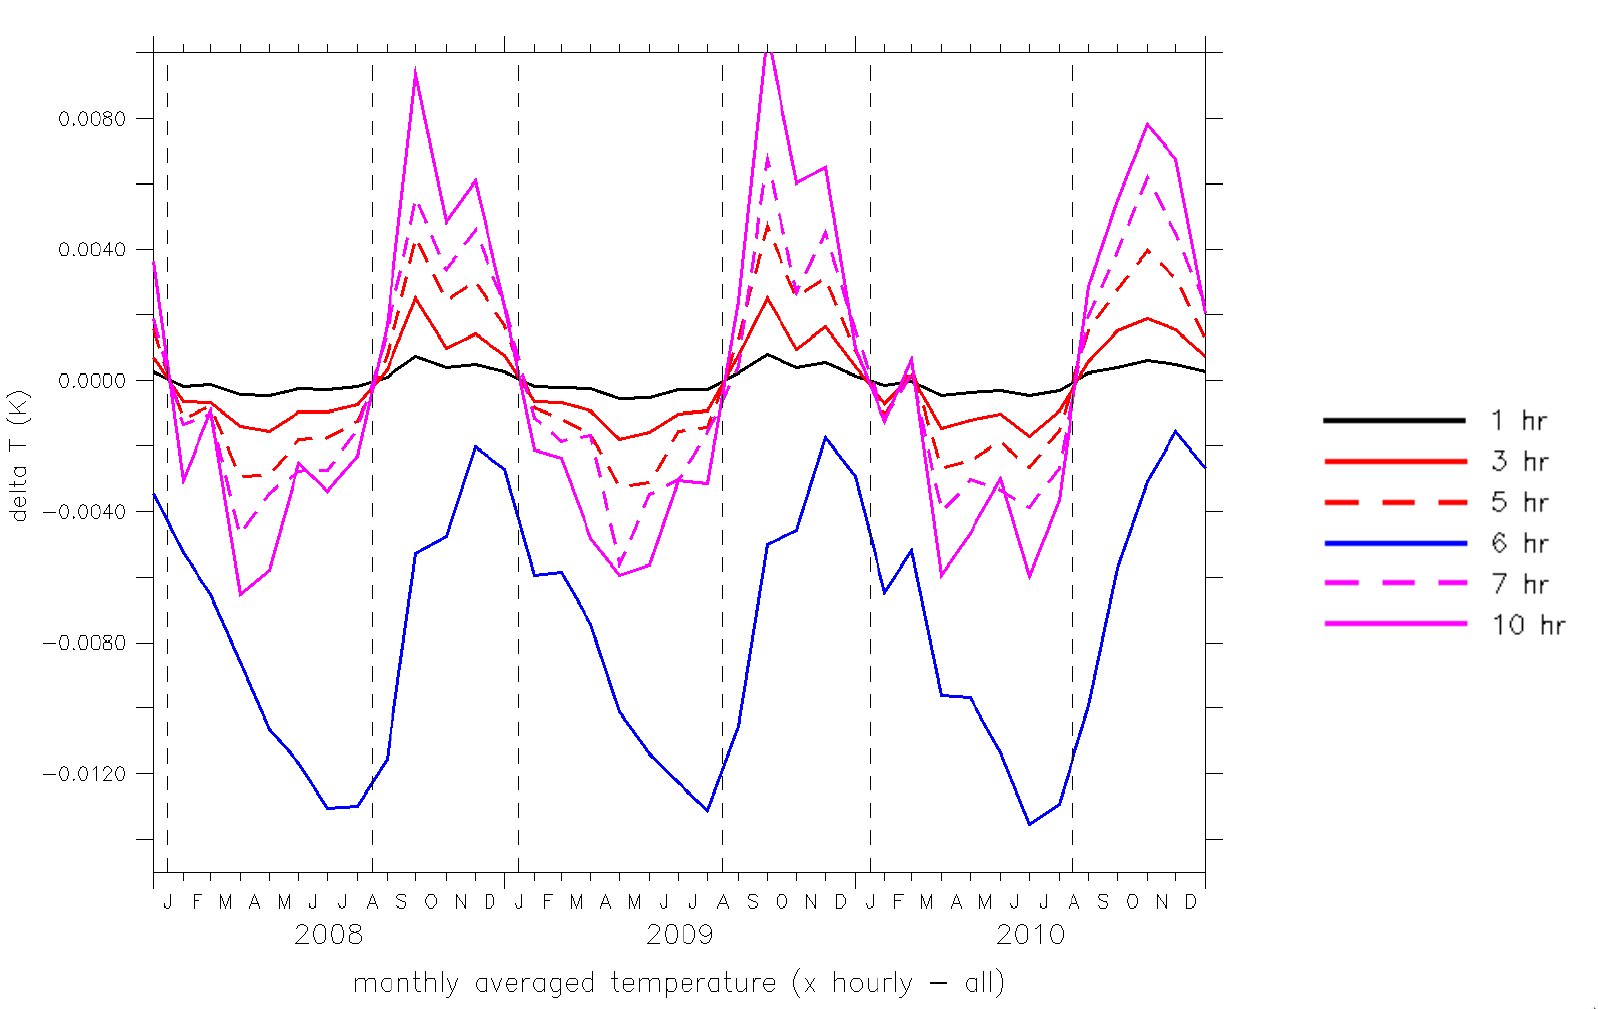
\includegraphics[width=0.7\textwidth]{EMAC_global_ll_temp}
  \caption{\label{fig:EMAC-glob-LL-temp} Globally averaged temperature in lowest
    model level. The differences of monthly averages based on different
    samples (``x-hourly'' - ``all'') are shown.}
  \end{center}
\end{figure*}

This bias is caused by systematic differences of the temperature over land.
This is shown in Figures \ref{fig:EMAC-glob-LL-land} and
\ref{fig:EMAC-glob-LL-sea}, which show the same results, however, for land and
sea separated, respectively.

\begin{figure*}
  \begin{center}
  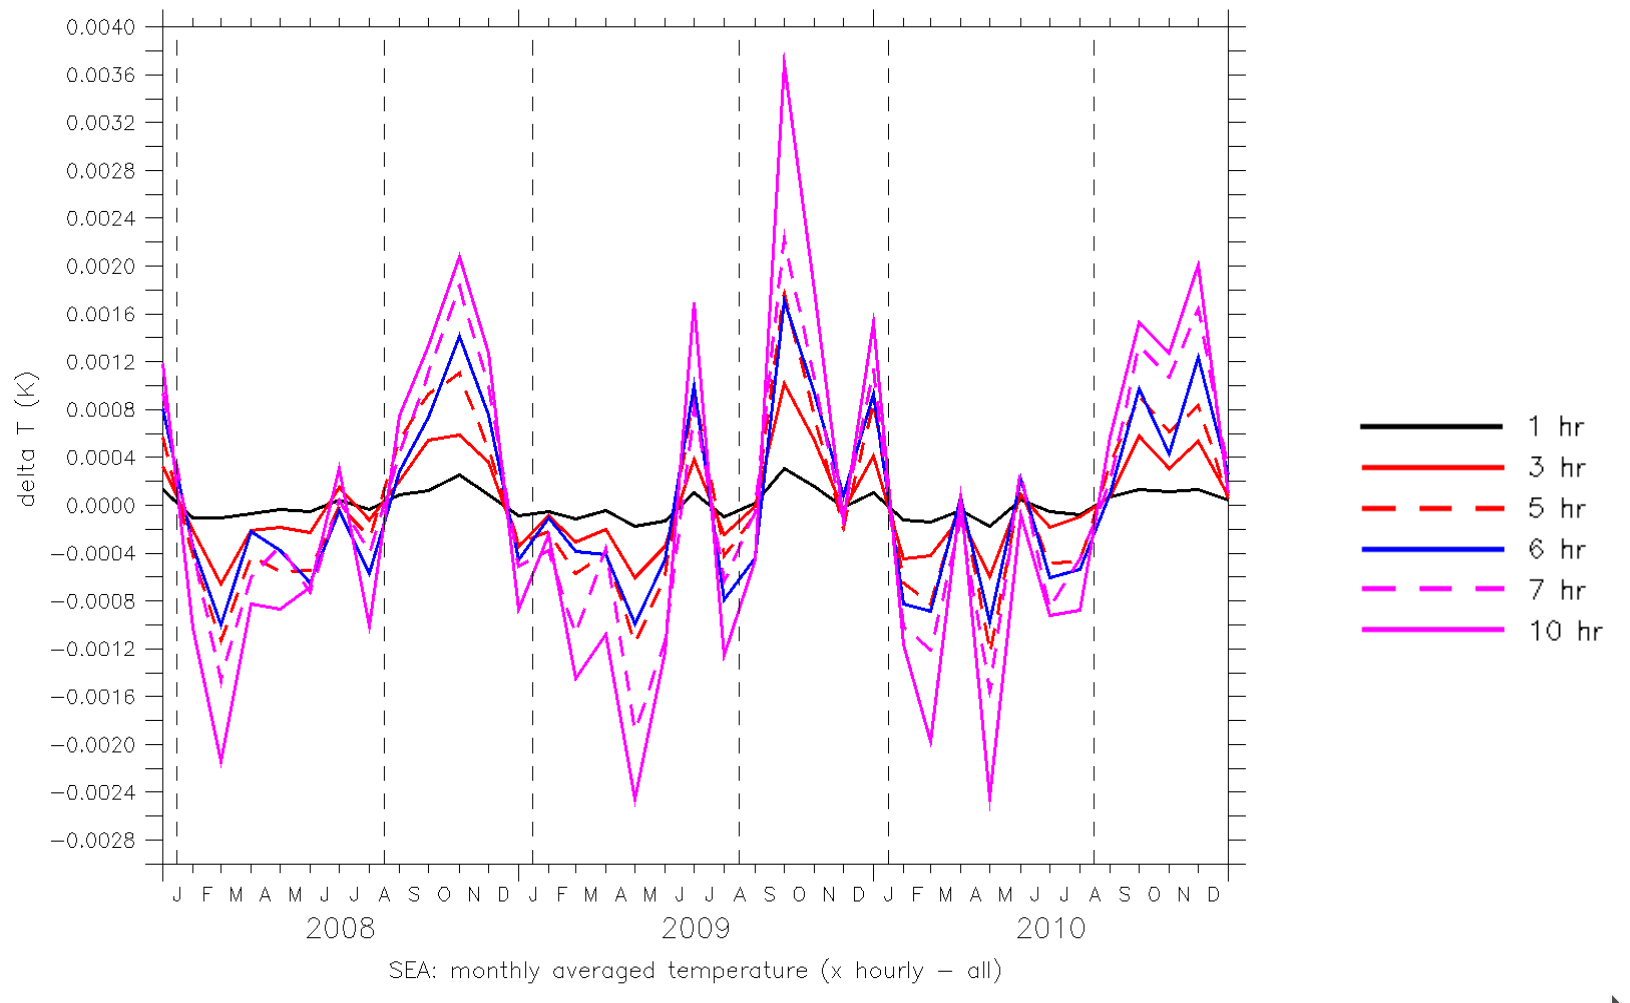
\includegraphics[width=0.7\textwidth]{EMAC_global_ll_temp_sea}
  \caption{\label{fig:EMAC-glob-LL-sea} Globally averaged temperature in
    lowest model level over sea only. The differences of monthly averages
    based on different samples (``x-hourly'' - ``all'') are shown.}
  \end{center}
\end{figure*}
\begin{figure*}
  \begin{center}
  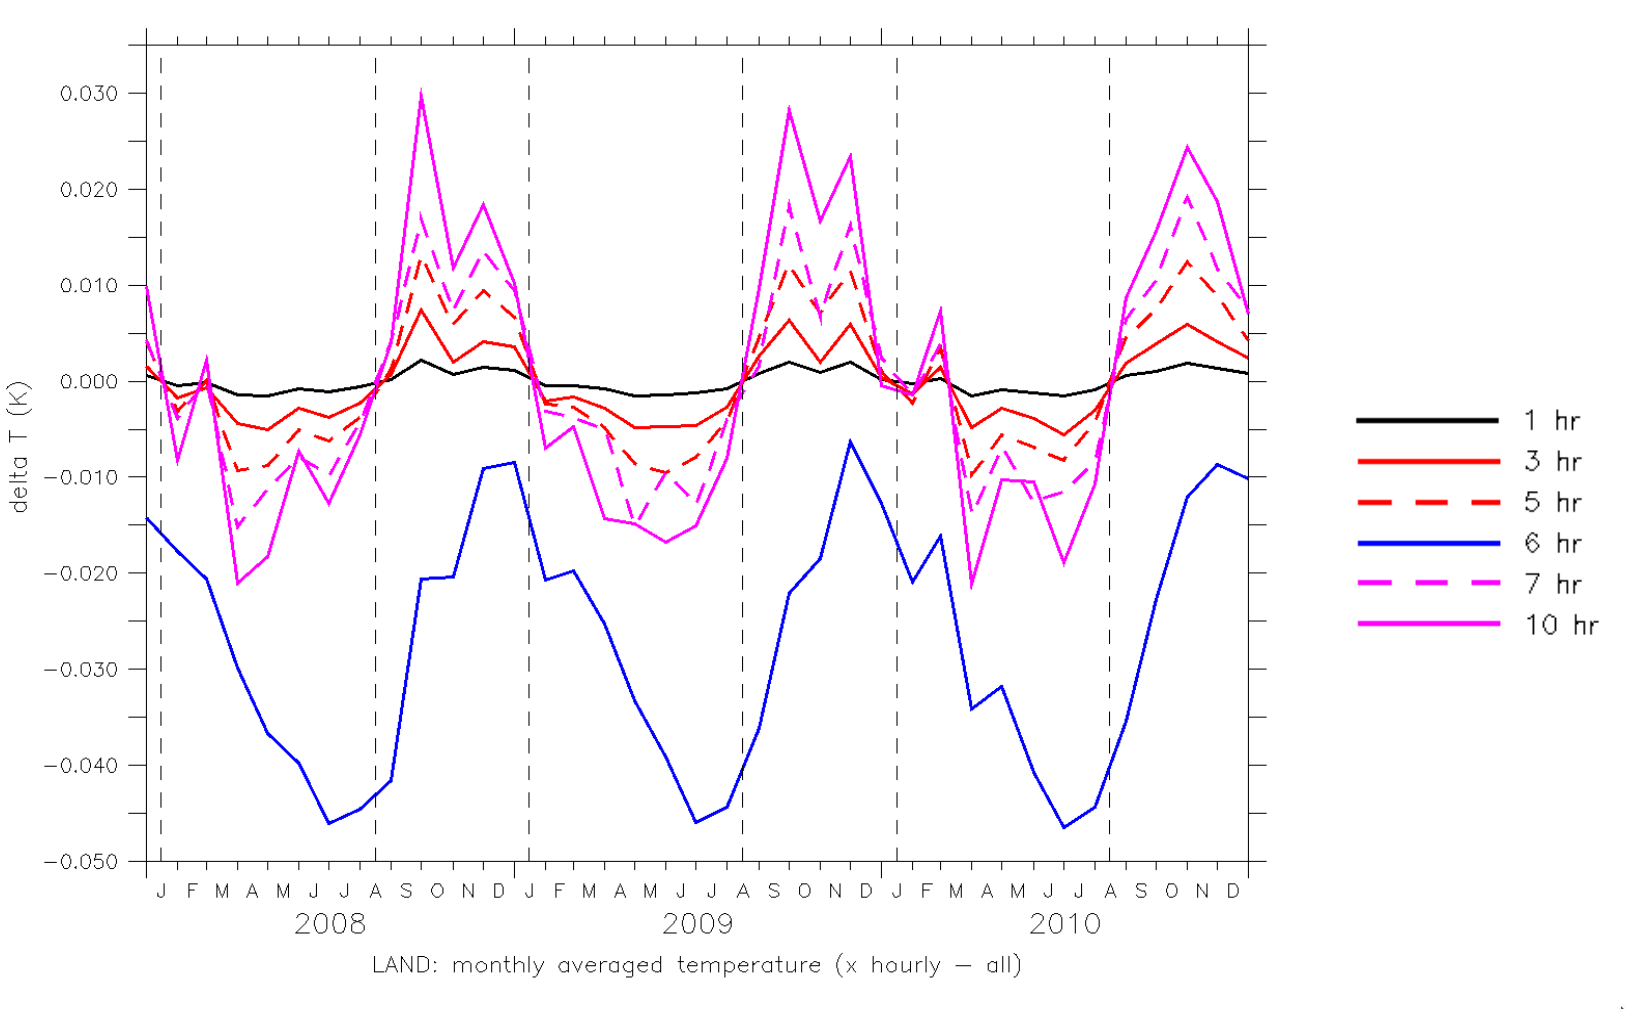
\includegraphics[width=0.7\textwidth]{EMAC_global_ll_temp_land}
  \caption{\label{fig:EMAC-glob-LL-land} Globally averaged temperature in lowest
    model level over land points only. The differences of monthly averages
    based on different samples (``x-hourly'' - ``all'') are shown.}
  \end{center}
\end{figure*}

Figure \ref{fig:EMAC-timeave} provides a global view of the differences of the
monthly temperature averages calculated with 6-hourly and all data,
respectively.  The sign of the bias depends on the
region. Furthermore, it depends on the off-set (shift of sampling)
of the 6-hourly data (not shown).
\begin{figure*}
  \begin{center}
  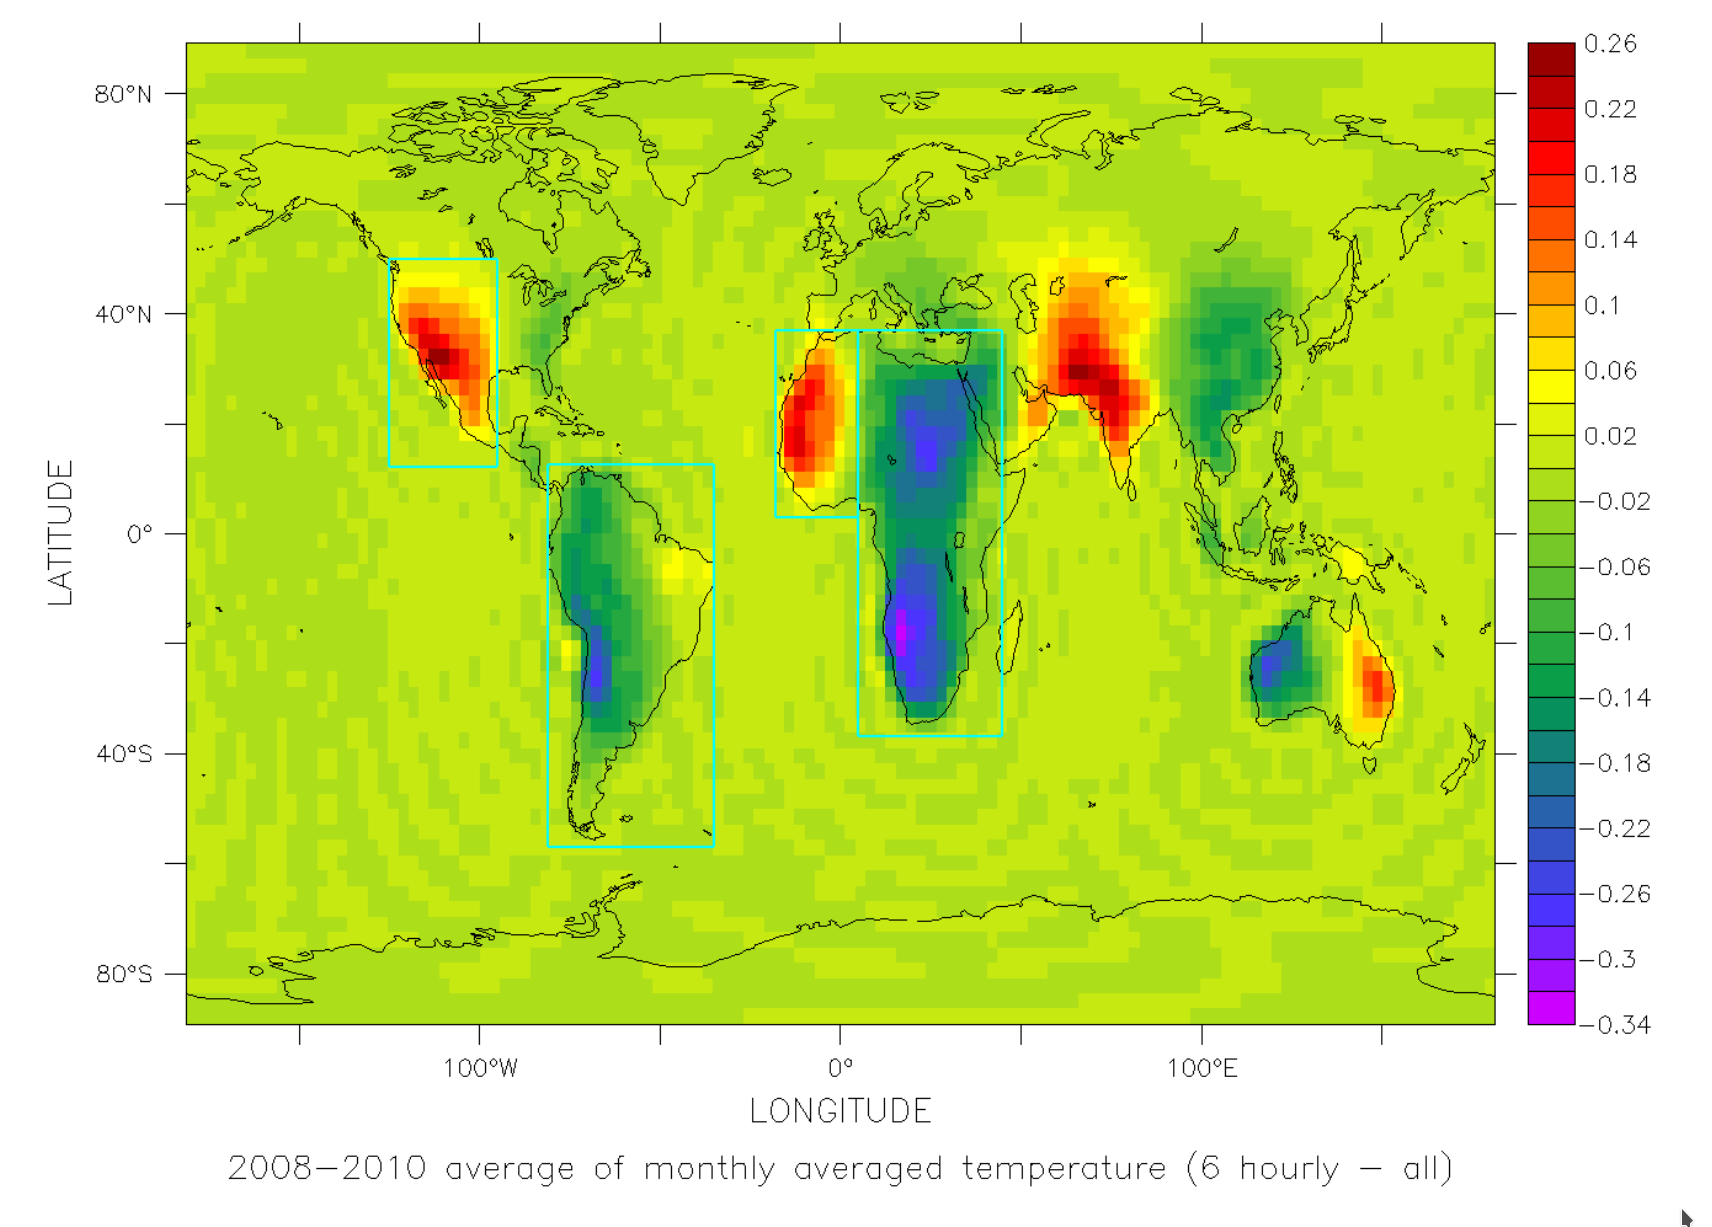
\includegraphics[width=0.7\textwidth]{EMAC_08-10ave_ll_temp_6hrly}
  \caption{\label{fig:EMAC-timeave} Time averaged (2008-2010) temperature in lowest
    model level. Differences of monthly averages based on different subsamples
    (``6-hourly'' - ``all'')
    are shown. The boxes indicate the regions used in
    Fig.\ \ref{fig:EMAC-4regions} for the area averages.}
  \end{center}
\end{figure*}

Figure \ref{fig:EMAC-4regions} illustrates exemplarily for the four regions
North and South America, North-West and East Africa that in individual
regions the bias induced by the usage of 6-hourly data can be as high as 0.2 K.

\begin{figure*}
  \begin{center}
  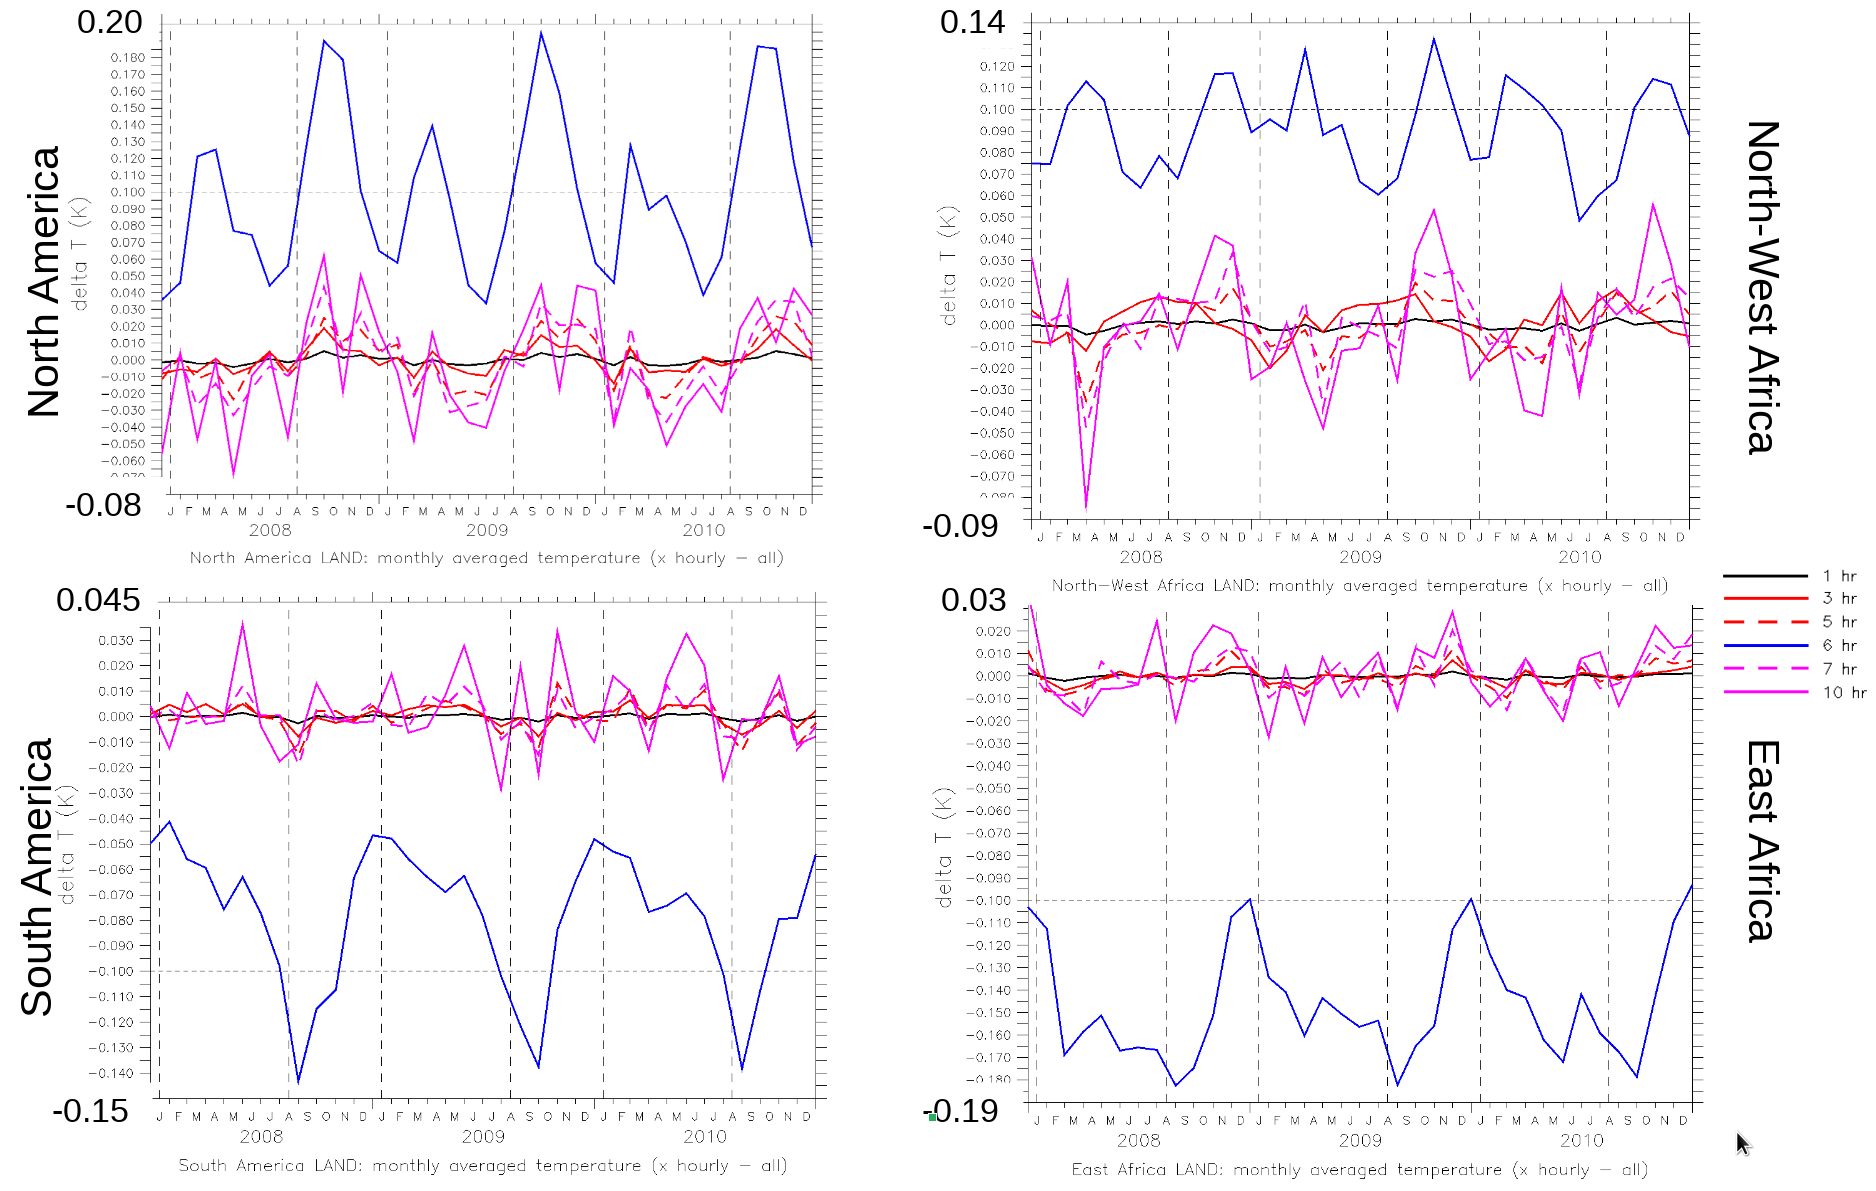
\includegraphics[width=0.7\textwidth]{EMAC-4regions}
  \caption{\label{fig:EMAC-4regions} Globally averaged temperature in lowest
    model level over land points. Differences of monthly averages
    based on different subsamples (``x-hourly'' - ``all'') are shown.}
  \end{center}
\end{figure*}


%%%%%%%%%%%%%%%%%%%%%%%%%%%%%%%%%%%%%%%%%%%%%%%%%%%%%%%%%%%%%%%%%%%%%%%%%%%%%%
%% ###########################################################################
%%%%%%%%%%%%%%%%%%%%%%%%%%%%%%%%%%%%%%%%%%%%%%%%%%%%%%%%%%%%%%%%%%%%%%%%%%%%%%

%%%%%%%%%%%%%%%%%%%%%%%%%%%%%%%%%%%%%%%%%%%%%%%%%%%%%%%%%%%%%%%%%%%%%%%%%%%%%%
%% ###########################################################################
%%%%%%%%%%%%%%%%%%%%%%%%%%%%%%%%%%%%%%%%%%%%%%%%%%%%%%%%%%%%%%%%%%%%%%%%%%%%%%
%%%%%%%%%%%%%%%%%%%%%%%%%%%%%%%%%%%%%%%%%%%%%%%%%%%%%%%%%%%%%%%%%%%%%%%%%%%%%%
%%\bibliographystyle{copernicus} % bst file
%%\bibliography{main_timer}  % bib file
%%%%%%%%%%%%%%%%%%%%%%%%%%%%%%%%%%%%%%%%%%%%%%%%%%%%%%%%%%%%%%%%%%%%%%%%%%%%%%
\end{document}


